\documentclass{article}
\usepackage{tikz}

\begin{document}

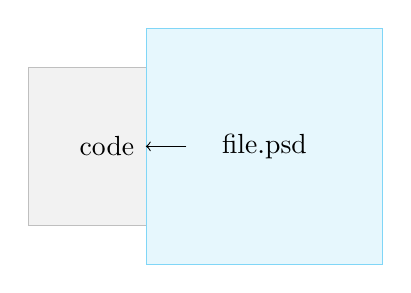
\begin{tikzpicture}[node distance=2cm]
    % Define nodes
    \node[draw=gray!50, fill=gray!10, rectangle, minimum width=2cm, minimum height=2cm] (code) {code};
    \node[draw=cyan!50, fill=cyan!10, rectangle, minimum width=3cm, minimum height=3cm, right of=code] (psd) {file.psd};
    
    % Draw line between nodes
    \draw[->] (code) -- (psd);
\end{tikzpicture}

\end{document}